

%% Slide 22.
\begin{frame}
\frametitle{Simulazione}
\begin{itemize}[<+->]
\item
La simulazione consiste in un'unica ``run'' del modello proposto;
\item
$180$ client che generano circa $80$--$90$ response per un totale dell'ordine delle
$15000$--$16000$ variabili;
\item
possibile utilizzare il metodo \emph{Batch}
per le stime statistiche, considerando ogni client un batch a sè stante.
\end{itemize}
\end{frame}

%% Slide 23.
\begin{frame}
\frametitle{Valutazioni}
\begin{block}{Valutare il DVE dal punto di vista della rete}
Focus su tre parametri:
\begin{itemize}%[<+->]
\item
\texttt{dveResponse},
\item
\texttt{clientMovesLost},
\item
\texttt{clientPresenceFactor}.
\end{itemize}
\end{block}
\pause
\vfill
\begin{exampleblock}{Un primo risultato notevole}
Il primo fatto che balza all'occhio analizzando i dati ottenuti è la totale
\alert{assenza di mosse perse} dai client.
\end{exampleblock}
\end{frame}

\subsection*{Tempo di risposta}

%% Slide 24.
\begin{frame}
\frametitle{Response Time}
\begin{figure}
\begin{center}
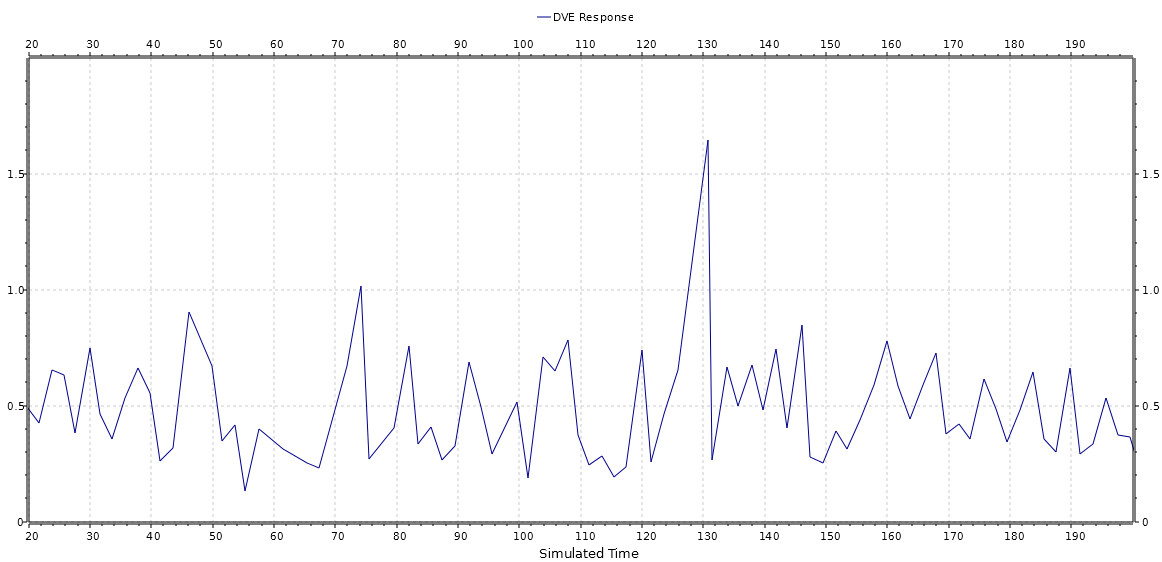
\includegraphics[scale=0.34]{response.jpeg}
\end{center}
\caption{Il \emph{Response Time} del client 175.}
\label{response}
\end{figure}
\end{frame}


%% Slide 25.
\begin{frame}
\frametitle{Analisi statistica}
I dati vengono suddivisi in 180 batch, in ciascuno sono quindi presenti un
numero $n_i$ variabile di osservazioni ($i \in \{1, \ldots, 180\}$).

All'interno del batch $i$ viene calcolata la media:
\[
\bar{X_i} = \frac{1}{n_i} \sum_{j=1}^{n_i} X_{ij}
\]

Si calcola quindi la stima puntuale della media:
\[
\hat{\mu} = \frac{1}{180}\sum_{i=1}^{180}\bar{X_i}
\]

Ed infine la varianza campionaria:
\[
S^2 = \frac{1}{179} \sum_{i=1}^{180}\left( \bar{X_i} - \hat{\mu}\right)^2
\]
\end{frame}

%% Slide 25.
\begin{frame}
\frametitle{Analisi statistica}
\begin{block}{Statistiche}
Esportando i dati ottenuti dalla simulazione in formato \texttt{CVS} è stato
possibile effettuare questi calcoli comodamente mediante uno script
\texttt{Phyton} con i seguenti risultati:
\begin{itemize}
\item
Stima puntuale della media $\hat{\mu} = 0.4993s$;
\item
Varianza campionaria $S^2 = 0.0008s$.
\end{itemize}
\end{block}
\pause
\vfill
\begin{exampleblock}{Intervallo di confidenza}
Con un livello di confidenza del $95$\% si ha il seguente intervallo di
confidenza:
\[
0.4928 \le \hat{\mu} \le 0.5058
\]
\end{exampleblock}
\end{frame}

\subsection*{Fattore presenze}

%% Slide 26.
\begin{frame}
\frametitle{Presence Factor}
\begin{figure}
\begin{center}
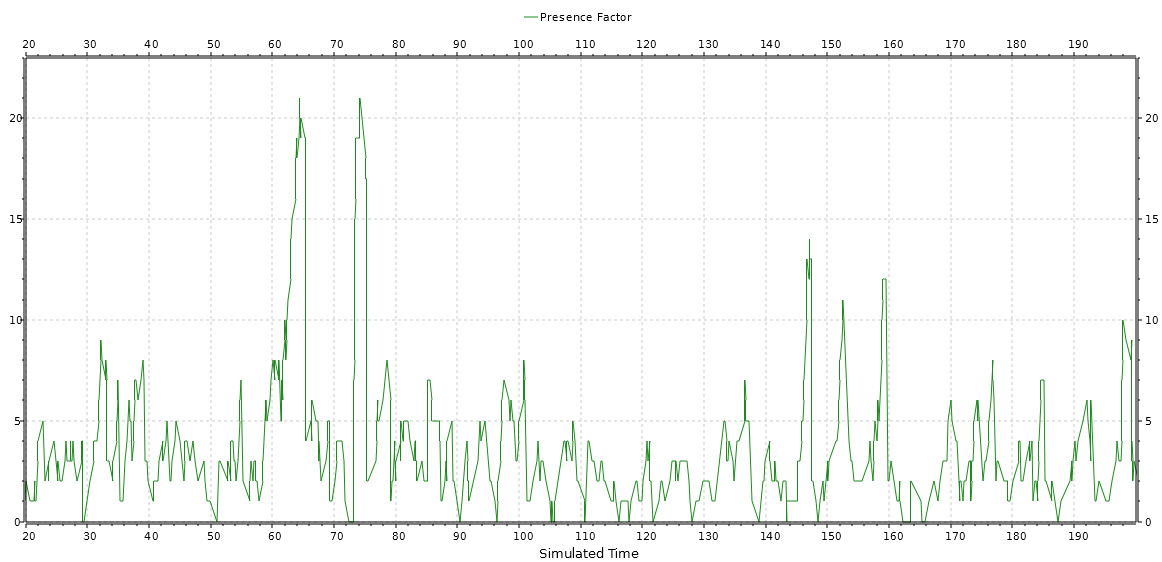
\includegraphics[scale=0.34]{presence.jpeg}
\end{center}
\caption{Il \emph{Presence Factor} del client 175.}
\label{presence}
\end{figure}
\end{frame}

%% Slide 27.
\begin{frame}
\frametitle{Presence Factor}
\begin{figure}
\begin{center}
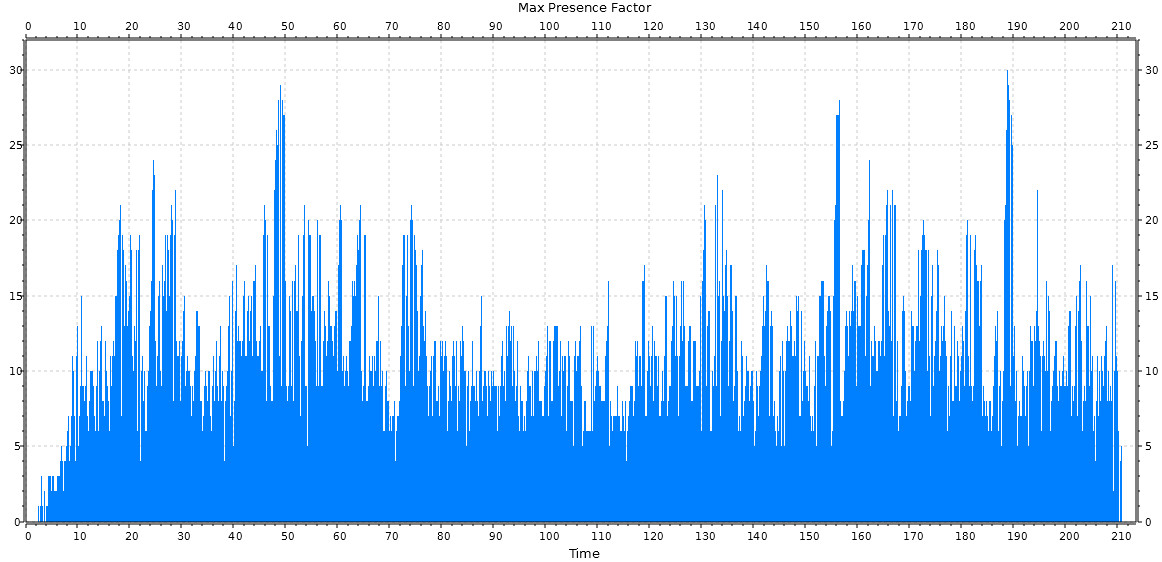
\includegraphics[scale=0.34]{maxPresenceFactor.jpeg}
\end{center}
\caption{Massimo valore di \emph{Presence Factor} dei client.}
\label{maxPresence}
\end{figure}
\end{frame}

%% Slide 28.
\begin{frame}
\frametitle{Relazione tra Response Time e
Presence Factor}
\begin{figure}
\begin{center}
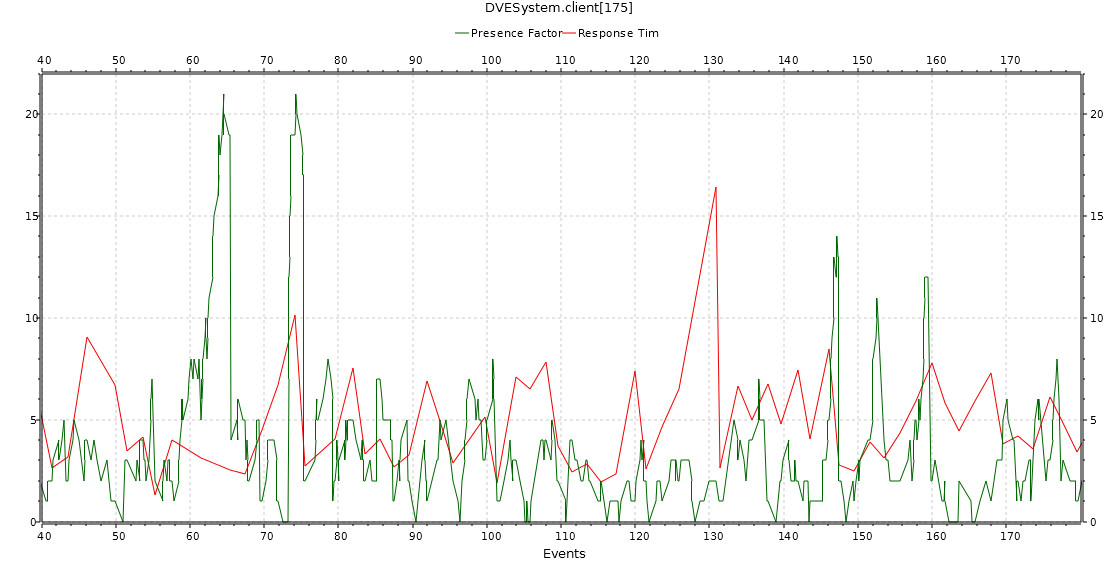
\includegraphics[scale=0.34]{responseVSpresence.jpeg}
\end{center}
\caption{Mancanza di correlazione tra \emph{Response Time} e
\emph{Presence Factor}.}
\label{responseVSPresence}
\end{figure}
\end{frame}

%% Slide 29.
\begin{frame}
\frametitle{Cosa accade aumentando gli uteni?}
\begin{block}{Statistiche}
Con $3$ server e $360$ client si evidenziano
i seguenti risultati:
\begin{itemize}
\item
Stima puntuale della media $\hat{\mu} = 0.5405s$;
\item
Varianza campionaria $S^2 = 0.0024s$.
\end{itemize}
\end{block}
\pause
\vfill
\begin{exampleblock}{Intervallo di confidenza}
Con un livello di confidenza del $95$\% si ha il seguente intervallo di
confidenza:
\[
0.5354 \le \hat{\mu} \le 0.5456
\]
\end{exampleblock}
\end{frame}
